@% Chapter 5

\chapter{Aplicação} % Main chapter title
\label{chap:Chapter5} % For referencing the chapter elsewhere, use \ref{chap:Chapter5} 

%----------------------------------------------------------------------------------------
\section{Sistema Desenvolvido}
O objetivo principal da parte prática da dissertação é não só recolher sinais e analisá-los, mas também criar a sua função de ambiguidade e verificar a presença do efeito de \textit{doppler} quando recebemos um sinal ao passar um objeto com uma \gls{RCS} significativa entre o transmissor e recetor.\par 
Para realizar estas tarefas foi utilizado um transmissor e recetor LimeSDR USB. As suas principais caraterísticas estão apresentadas na seguinte tabela e a sua documentação em \url{https://wiki.myriadrf.org/LimeSDR-USB}.\par

\begin{table}[h]
\centering
\begin{tabular}{@{}ccccc@{}}
\toprule
Caraterística       			 & Descrição                      \\ \midrule
\textit{RF Transreceiver}        & LMS7002M                       \\
\textit{Oscillator}    			 & Rakon RPT7050A @30.72 $MHz$    \\
Banda de frequência              & 100$kHz$ - 3.8$GHz$            \\ 
Largura de banda máxima          & 61.44$MHz$                     \\ \bottomrule
\label{tab:limesdr}
\end{tabular}
\caption[Caraterísticas do LimeSDR USB]{Caraterísticas do LimeSDR USB}
\end{table}

Por forma a reduzir o ruído a alimentação é feita através dum \textit{power bank} de 20000$mAh$. Isto é conseguido com um cabo em "Y" que vem com o LimeSDR, que separa a entrada de dados da alimentação do equipamento.

Como falado durante os diversos capítulos desta dissertação, a função de ambiguidade permite conhecer o sinal recebido e a sua distorção provocada pelo fitro adaptado, falado com mais pormenor no capítulo \ref{chap:Chapter4}. \par
Assim, utilizando o matlab e as ferramentas que este dispõe, é possível calcular funções de ambiguidade de diversos sinais, tendo como um exemplo a figura \ref{fig:ambfun_fmdef} que é resultado do código em anexo \ref{Annex1} apresentado pelo matlab para fazer funções de ambiguidade consoante as caraterísticas do sinal.
\begin{figure}[h]
\centering
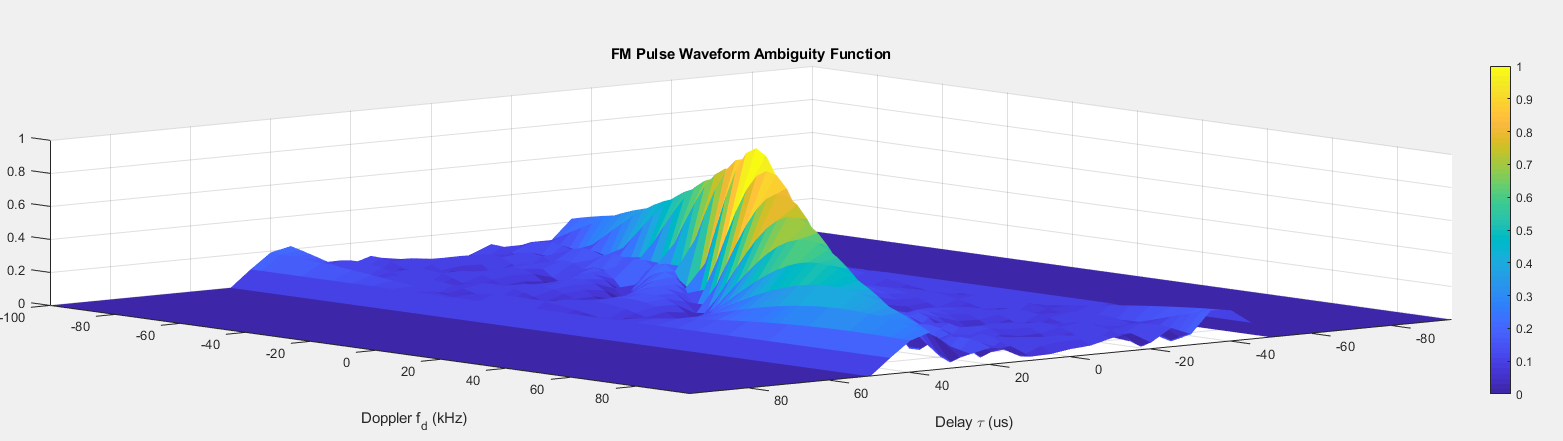
\includegraphics[scale=0.4]{chapters/ch5/assets/ambfun_fmdef}
\caption[Função de ambiguidade para um pulso FM]{Função de ambiguidade para um pulso FM}
\label{fig:ambfun_fmdef}
\end{figure}


\begin{figure}[h]
\centering
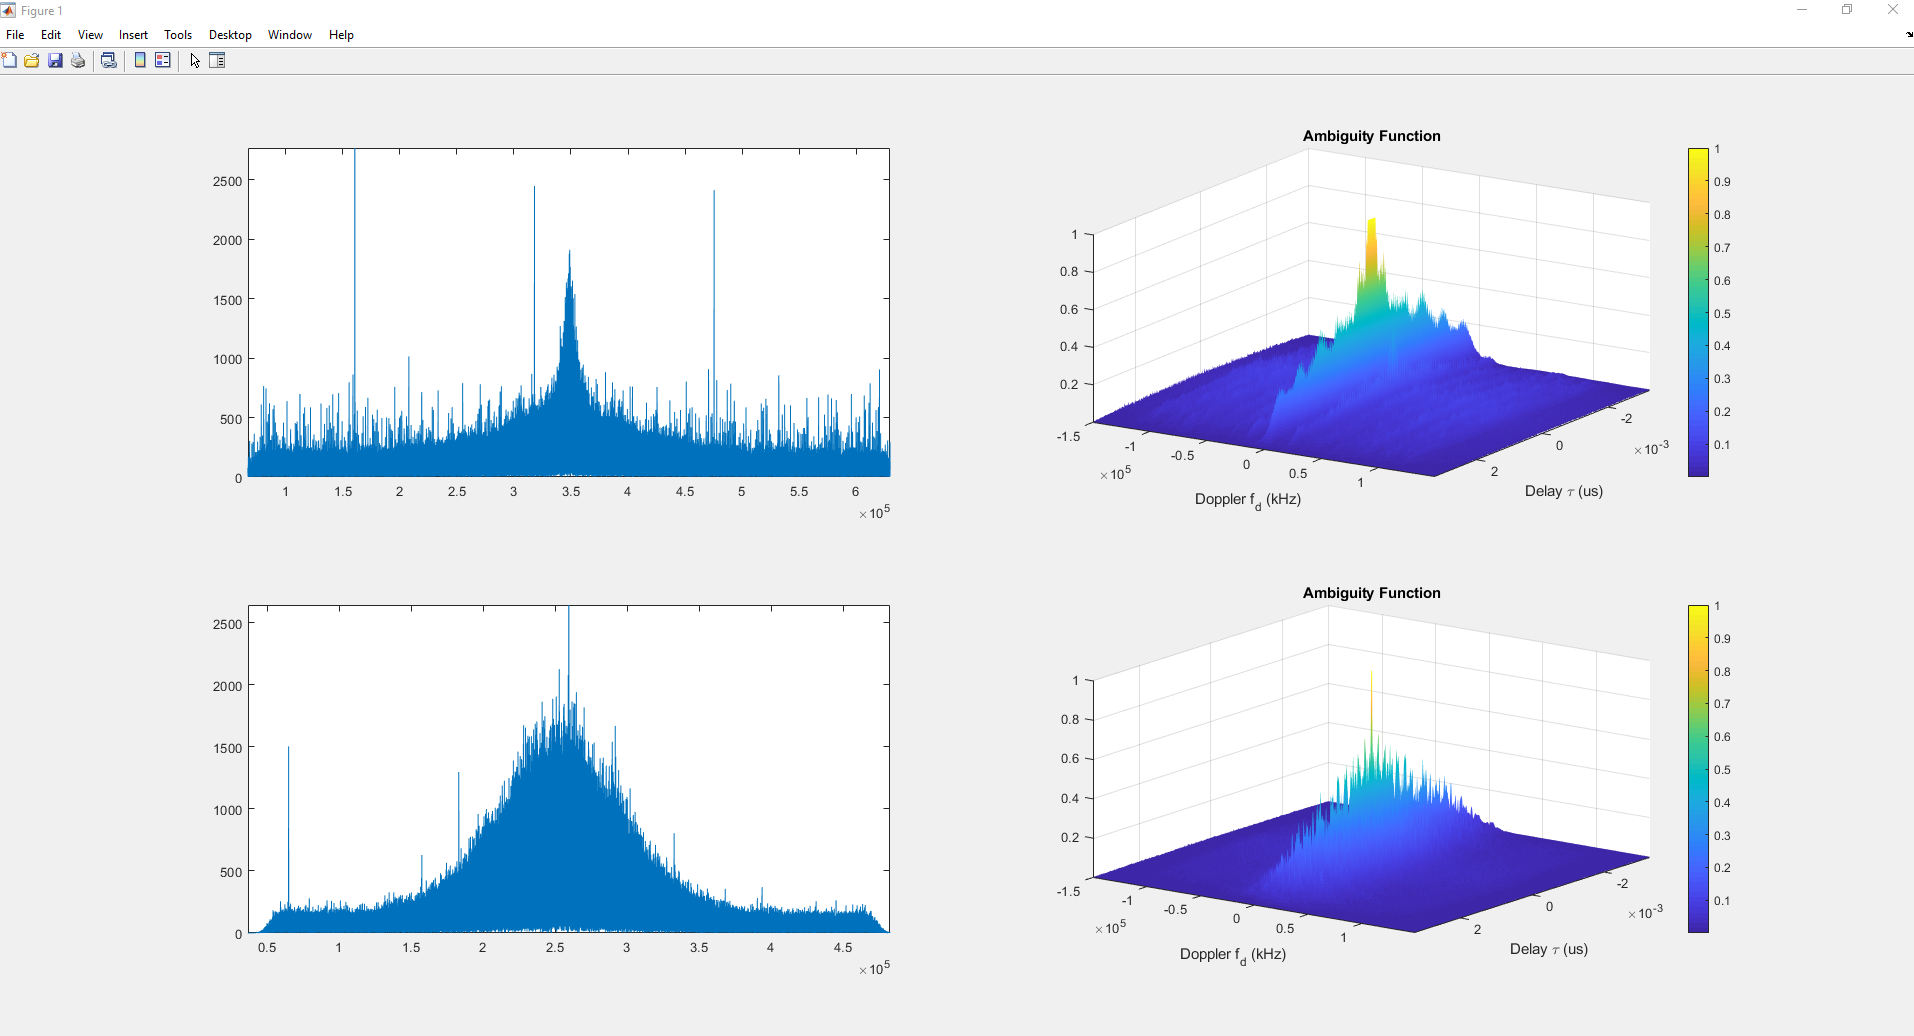
\includegraphics[scale=0.3]{chapters/ch5/assets/ambfun2}
\caption[Função de ambiguidade para uma estação FM]{Função de ambiguidade para um pulso FM retirada de uma estação a dar notícias e música pop}
\label{fig:ambfun2}
\end{figure}
 


\section{Resultados}


